\appendix

\chapter{Machine Learning Model} \label{ap:model}
\begin{lstlisting}[language=Python]
inp = Input((28,28))
out = Reshape((28,28,1))(inp)
out = Conv2D(16, (3,3), activation="relu")(out)
out = Conv2D(16, (3,3), activation="relu")(out)
out = Flatten()(out)
out = Dense(128, activation="relu")(out)
out = Dense(10, activation="sigmoid")(out)
model = Model(inputs=inp, outputs=out)
model.compile(
	optimizer="adam",
	loss=SparseCategoricalCrossentropy(),
	metrics=[SparseCategoricalAccuracy()])
\end{lstlisting}

\chapter{Gantt Charts}
\newpage
\section{Gantt - Interim} \label{gc-interim}
\begin{center}
	\rotatebox[origin=c]{-90}{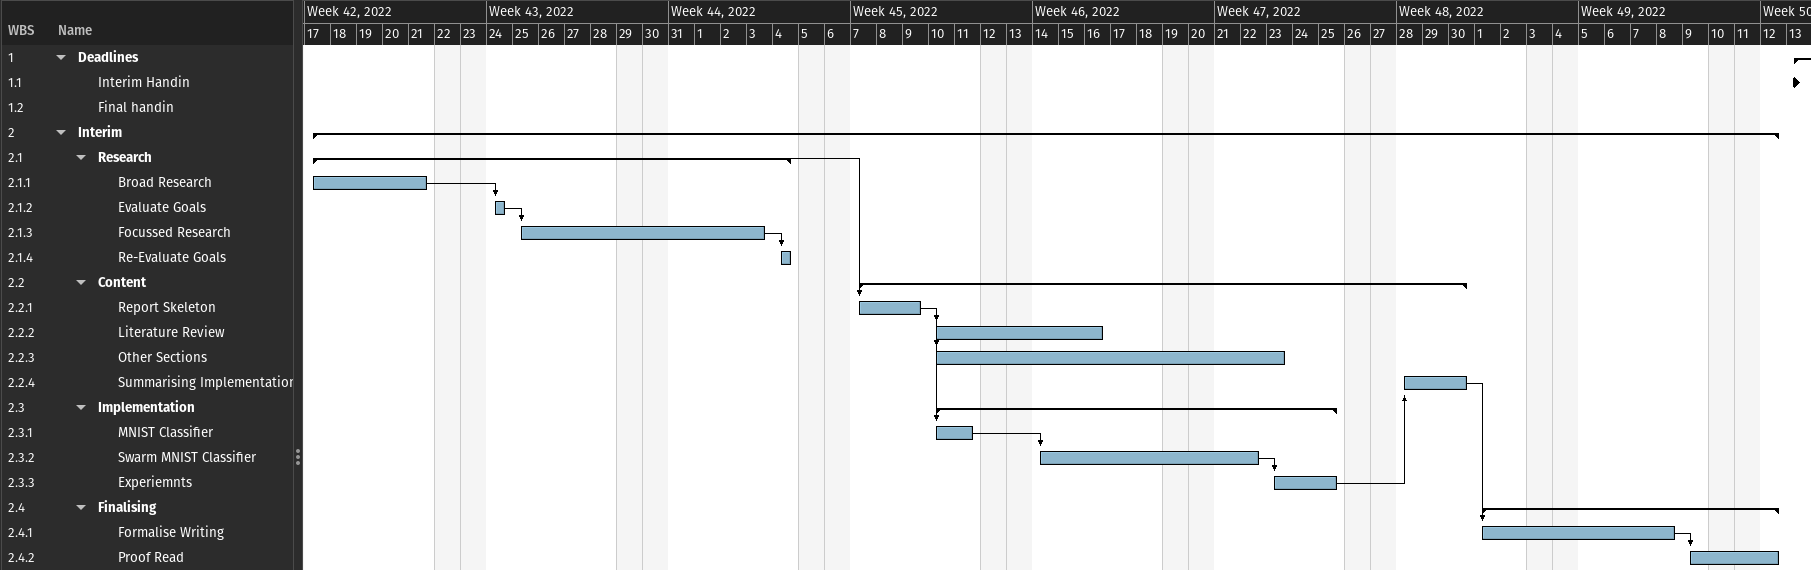
\includegraphics[width=\textheight]{gannt-interim}}
\end{center}

\section{Gantt - Final} \label{gc-final}
\begin{center}
	\rotatebox[origin=c]{-90}{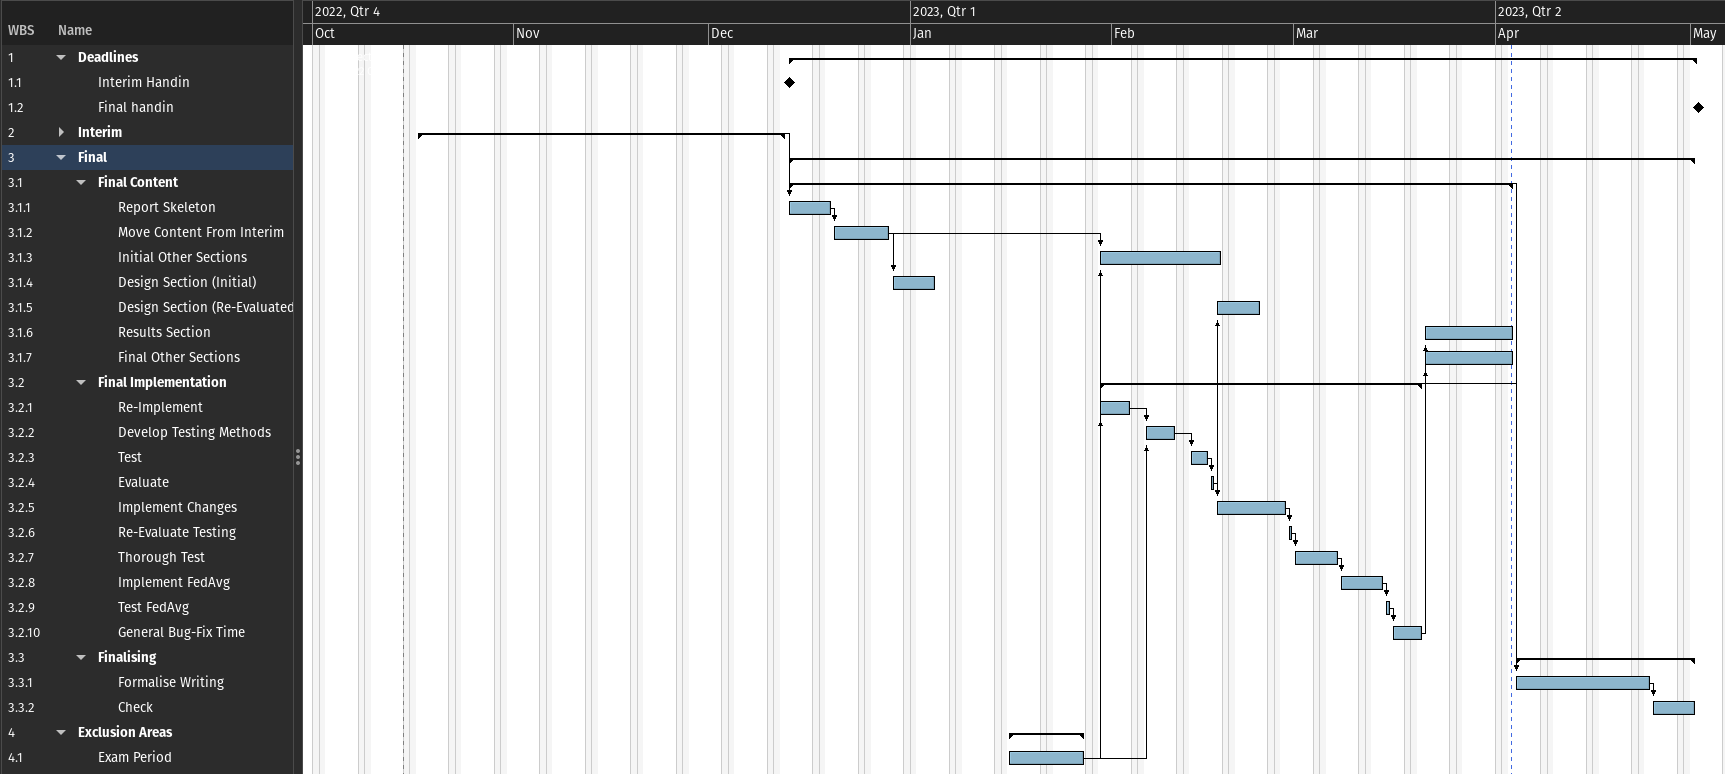
\includegraphics[width=\textheight]{gannt-final}}
\end{center}